% Options for packages loaded elsewhere
\PassOptionsToPackage{unicode}{hyperref}
\PassOptionsToPackage{hyphens}{url}
\PassOptionsToPackage{dvipsnames,svgnames,x11names}{xcolor}
%
\documentclass[
  11pt,
]{article}
\usepackage{amsmath,amssymb}
\usepackage{lmodern}
\usepackage{iftex}
\ifPDFTeX
  \usepackage[T1]{fontenc}
  \usepackage[utf8]{inputenc}
  \usepackage{textcomp} % provide euro and other symbols
\else % if luatex or xetex
  \usepackage{unicode-math}
  \defaultfontfeatures{Scale=MatchLowercase}
  \defaultfontfeatures[\rmfamily]{Ligatures=TeX,Scale=1}
\fi
% Use upquote if available, for straight quotes in verbatim environments
\IfFileExists{upquote.sty}{\usepackage{upquote}}{}
\IfFileExists{microtype.sty}{% use microtype if available
  \usepackage[]{microtype}
  \UseMicrotypeSet[protrusion]{basicmath} % disable protrusion for tt fonts
}{}
\makeatletter
\@ifundefined{KOMAClassName}{% if non-KOMA class
  \IfFileExists{parskip.sty}{%
    \usepackage{parskip}
  }{% else
    \setlength{\parindent}{0pt}
    \setlength{\parskip}{6pt plus 2pt minus 1pt}}
}{% if KOMA class
  \KOMAoptions{parskip=half}}
\makeatother
\usepackage{xcolor}
\usepackage[left=1in,right=1in,top=1in,bottom=1in]{geometry}
\usepackage{longtable,booktabs,array}
\usepackage{calc} % for calculating minipage widths
% Correct order of tables after \paragraph or \subparagraph
\usepackage{etoolbox}
\makeatletter
\patchcmd\longtable{\par}{\if@noskipsec\mbox{}\fi\par}{}{}
\makeatother
% Allow footnotes in longtable head/foot
\IfFileExists{footnotehyper.sty}{\usepackage{footnotehyper}}{\usepackage{footnote}}
\makesavenoteenv{longtable}
\usepackage{graphicx}
\makeatletter
\def\maxwidth{\ifdim\Gin@nat@width>\linewidth\linewidth\else\Gin@nat@width\fi}
\def\maxheight{\ifdim\Gin@nat@height>\textheight\textheight\else\Gin@nat@height\fi}
\makeatother
% Scale images if necessary, so that they will not overflow the page
% margins by default, and it is still possible to overwrite the defaults
% using explicit options in \includegraphics[width, height, ...]{}
\setkeys{Gin}{width=\maxwidth,height=\maxheight,keepaspectratio}
% Set default figure placement to htbp
\makeatletter
\def\fps@figure{htbp}
\makeatother
\setlength{\emergencystretch}{3em} % prevent overfull lines
\providecommand{\tightlist}{%
  \setlength{\itemsep}{0pt}\setlength{\parskip}{0pt}}
\setcounter{secnumdepth}{5}
\usepackage{setspace}
\usepackage{float}
\usepackage{mathtools}
\usepackage{natbib}
\usepackage[linesnumbered,ruled,vlined]{algorithm2e}
\setcitestyle{year,comma}
\usepackage{verbatim}
\usepackage{amsthm}
\usepackage{comment}
\ifLuaTeX
  \usepackage{selnolig}  % disable illegal ligatures
\fi
\usepackage[]{natbib}
\bibliographystyle{apalike}
\IfFileExists{bookmark.sty}{\usepackage{bookmark}}{\usepackage{hyperref}}
\IfFileExists{xurl.sty}{\usepackage{xurl}}{} % add URL line breaks if available
\urlstyle{same} % disable monospaced font for URLs
\hypersetup{
  colorlinks=true,
  linkcolor={Maroon},
  filecolor={Maroon},
  citecolor={Blue},
  urlcolor={blue},
  pdfcreator={LaTeX via pandoc}}

\author{}
\date{\vspace{-2.5em}}

\usepackage{amsthm}
\newtheorem{theorem}{Theorem}[section]
\newtheorem{lemma}{Lemma}[section]
\newtheorem{corollary}{Corollary}[section]
\newtheorem{proposition}{Proposition}[section]
\newtheorem{conjecture}{Conjecture}[section]
\theoremstyle{definition}
\newtheorem{definition}{Definition}[section]
\theoremstyle{definition}
\newtheorem{example}{Example}[section]
\theoremstyle{definition}
\newtheorem{exercise}{Exercise}[section]
\theoremstyle{definition}
\newtheorem{hypothesis}{Hypothesis}[section]
\theoremstyle{remark}
\newtheorem*{remark}{Remark}
\newtheorem*{solution}{Solution}
\begin{document}

\doublespacing

\pagenumbering{gobble}

%\begin{titlepage}
\begin{center}
\LARGE{\textsc{Community Detection in the Setting of Generalized Random Dot Product Graphs}}\\
\vspace*{6\baselineskip}
\normalsize{John Koo}\\
\vspace*{10\baselineskip}
\singlespacing
\normalsize{Submitted to the faculty of the Univesity Graduate School \\
in partial fulfillment of the requirements for the degree \\
Doctor of Philosophy \\
in the Department of Statistics, \\
Indiana University \\
December 2022}
\vspace*{3\baselineskip}

\end{center}

\pagenumbering{roman}
\thispagestyle{empty}

\newpage

\singlespacing

Accepted by the Graduate Faculty, Indiana University, in partial fulfillment of the requirements for the degree of Doctor of Philosophy.

\vspace*{6\baselineskip}

\begin{tabular}{@{}p{1in}p{4in}@{}}
Approved: & \hrulefill \\
& Michael W. Trosset, Ph.D. \\
\\
\\
& \hrulefill \\
& Minh Tang, Ph.D. \\
\\
\\
& \hrulefill \\
& Julia Fukuyama, Ph.D. \\
\\
\\
& \hrulefill \\
& Roni Khardon, Ph.D. \\
\\
\\
& \hrulefill \\
& Fangzheng Xie, Ph.D. \\
\end{tabular}

\vspace*{16\baselineskip}

\raggedright

December 1, 2022

\newpage

\doublespacing

\begin{center}
\LARGE{\bf{Acknowledgements}}
\end{center}

\hypersetup{linkcolor = black}

\newpage

\begin{center}
\LARGE{Abstract}
\end{center}

\vspace*{2\baselineskip}

\normalsize

Graph and network data, in which samples are represented not as a collection of feature vectors but as relationships between pairs of observations, are increasingly widespread in various fields ranging from sociology to computer vision. One common goal of analyzing graph data is community detection or graph clustering, in which the graph is partitioned into disconnected subgraphs in an unsupervised yet meaningful manner (e.g., by optimizing an objective function or recovering unobserved labels). Because traditional clustering techniques were developed for data that can be represented as vectors, they cannot be applied directly to graphs. In this research, we investigate the use of a family of spectral decomposition based approaches for community detection in block models (random graph models with inherent community structure), first by demonstrating how under the Generalized Random Dot Product Graph framework, all graphs generated by block models can be represented as feature vectors, then applying clustering methods for these feature vector representations, and finally deriving the asymptotic properties of these methods. 

\newpage
\tableofcontents
\addcontentsline{toc}{section}{\contentsname}

\newpage
\pagenumbering{arabic}
\hypersetup{linkcolor = blue}

{
\hypersetup{linkcolor=}
\setcounter{tocdepth}{2}
\tableofcontents
}
\setlength{\parindent}{10.0pt}
\newcommand{\diag}{\mathrm{diag}}
\newcommand{\tr}{\mathrm{Tr}}
\newcommand{\blockdiag}{\mathrm{blockdiag}}
\newcommand{\indep}{\stackrel{\mathrm{ind}}{\sim}}
\newcommand{\iid}{\stackrel{\mathrm{iid}}{\sim}}
\newcommand{\Bernoulli}{\mathrm{Bernoulli}}
\newcommand{\Betadist}{\mathrm{Beta}}
\newcommand{\BG}{\mathrm{BernoulliGraph}}
\newcommand{\Uniform}{\mathrm{Uniform}}
\newcommand{\PABM}{\mathrm{PABM}}
\newcommand{\RDPG}{\mathrm{RDPG}}
\newcommand{\GRDPG}{\mathrm{GRDPG}}
\newcommand{\Multinomial}{\mathrm{Multinomial}}
\newcommand{\dd}{\mathrm{d}}
\newcommand{\as}{\stackrel{\mathrm{a.s.}}{\to}}
\newcommand{\ER}{\text{Erd\"{o}s-R\'{e}nyi}}
\newcommand{\SBM}{\mathrm{SBM}}
\newcommand{\DCBM}{\mathrm{DCBM}}
\newcommand{\argmin}{\mathrm{argmin}}

\hypertarget{introduction}{%
\section{Introduction}\label{introduction}}

\hypertarget{graphs-and-representations-of-network-data}{%
\subsection{Graphs and Representations of Network Data}\label{graphs-and-representations-of-network-data}}

Graph and network data have become increasingly widespread in various fields including sociology, neuroscience, biostatistics, and computer science.
This has resulted in challenges for researchers who rely on traditional statistical and machine learning methods that are incompatible with graph data and instead assume that the data exist as feature vectors.
To illustrate this, consider the typical approach to building a statistical or machine learning model.
Data are often represented as an \(n \times p\) matrix \(X = \begin{bmatrix} x_1 & \cdots & x_n \end{bmatrix}^\top\) in which each row \(x_i \in \mathbb{R}^p\) is an observation of \(p\) features and each column is a set of \(n\) feature measurements.
An analysis task for these data might be to come up with a classification model \(\phi : \mathbb{R}^p \to \{1, 2, ..., K\}\) that uses the numerical values of each feature of a vector \(x_i\) to calculate a predicted label \(z_i \in \{1, 2, ..., K\}\).
For instance, \(\phi(x)\) might first compute the distances from \(x\) to \(K\) points in \(\mathbb{R}^p\) and then assign \(x\) to the label of the nearest point.
Examples of this include linear discriminant analysis (in the case of supervised learning) and Lloyd's algorithm \citep{1056489} or Gaussian mixture models \citep{doi:10.1198/016214502760047131} (in the case of unsupervised learning).
However, it is not obvious how this method would translate to data that are represented as graphs, in which observations consist of relationships among a set of objects rather than numerical attributes associated with each object:
Instead of feature vector \(x_i = \begin{bmatrix} x_{i1} & \cdots & x_{ip} \end{bmatrix}^\top \in \mathbb{R}^p\), we observe \(a_i = \begin{bmatrix} a_{i1} & \cdots & a_{in} \end{bmatrix}^\top \in \mathbb{R}^n\) in which each \(a_{ij}\) is object \(i\)'s relationship to object \(j\).
For such data, it is often necessary to alter existing algorithms, transform the graph data into Euclidean data, often called \emph{graph embedding} or \emph{spectral clustering} \citep{vonLuxburg2007}, and apply algorithms for Euclidean data on the embedding, or come up with new algorithms altogether.

\begin{example}
$K$-means clustering \citep{MacQueen1967} is a nonparametric clustering method that minimizes the objective function
\begin{equation}
\label{eq:kmeans}
W(x_1, ..., x_n) = \sum_{k = 1}^K \sum_{x_i : z_i = k} \|x_i - \bar{x}_k\|_2^2,
\end{equation}
in which $x_1, ..., x_n \in \mathbb{R}^p$ are feature vectors of a sample, $z_1, ..., z_n \in \{1, ..., K\}$ are cluster assignments we wish to optimize for, and $\bar{x}_1, ..., \bar{x}_K \in \mathbb{R}^p$ are the centroids of each cluster, which act as nuisance parameters. 
A popular implementation of $K$-means clustering is Lloyd's algorithm \citep{1056489}, which is a type of coordinate descent algorithm in which at each iteration labels are updated according to which centroid they are closest to and centroids are updated via the sample mean of each cluster. 

If instead of vectors in $\mathbb{R}^p$ we have a graph, it is not obvious how to translate $K$-means clustering to these data. 
In particular, there is no inherent notion of centroid or sample mean for graph data. 
However, there are inherent notions of distances among vectors, such as shortest path distance, expected commute time, or resistance distance. 
One way to adapt $K$-means to graph data is to use an equivalent objective function as Eq.~\ref{eq:kmeans} that doesn't use centroids (which are just nuisance parameters) and is stated only in terms of distances:  
$$
\tilde{W}(x_1, ..., x_n) = \sum_{k=1}^K \sum_{x_i, x_j : z_i = z_j = k} d(x_i, x_j)^2.
$$
Here, $d(x_i, x_j)$ is the distance between objects $x_i$ and $x_j$. 
If the data live in a Euclidean vector space, then $d(x_i, x_j) = \|x_i - x_j\|_2$, 
or if the data are represented as a graph, then $d(x_i, x_j)$ represents some notion of graph distance. 
While this formulation of $K$-means clustering takes care of the lack of centroids, the implementation still requires some thought since Lloyd's algorithm includes the computation of centroids. 
An alternative algorithm is MacQueen's exchange algorithm \citep{MacQueen1967}, which involves cycling through each vertex and then, for each vertex, cycling through the labels and choosing the label that minimizes the objective function. 

Yet another approach to adapting $K$-means clustering to graph data is to embed the graph to Euclidean space and then apply Lloyd's algorithm on the embedding. 
\end{example}

We now provide a more formal description of graph data:
Suppose we observe a network of \(n\) objects and pairwise relationships between them.
This network is represented by a graph \(G = (V, E)\) with vertex set \(V = \{v_1, ..., v_n\}\), representing the \(n\) objects, and edge set \(E\), representing the up to \(n (n - 1) / 2\) pairwise relationships (assuming that there are no self-loops).
The numeric representation of these data is in the form of \emph{affinity matrix} \(A \in \mathbb{R}^{n \times n}\) in which each \(A_{ij}\) represents object \(i\)'s relationship to object \(j\).
We assume that the entries of \(A\) represent affinities or similarities, i.e., the higher the value of \(A_{ij}\), the stronger the relationship \(i\) has to \(j\).
If \(A_{ij} = 0\), then \(i\) has no direct relationship to \(j\).
\(A\) is symmetric if it represents an undirected graph in which the relationship from \(i\) to \(j\) is the same as the relationship from \(j\) to \(i\).
\(A\) is binary, i.e., \(A \in \{0, 1\}^{n \times n}\), if it represents an unweighted graph in which edges either exist or don't exist.
If \(A\) is binary, we call it an \emph{adjacency matrix}.

\begin{example}
\label{ex:uk-faculty}
\citet{PhysRevE.77.016107} constructed a friendship network among $81$ faculty from various schools at a university in the UK. 
These data are represented as a graph in which each vertex is a faculty member and edges between pairs of vertices indicate whether the two faculty are friends. 
The corresponding adjacency matrix $A \in \{0, 1\}^{81 \times 81}$ has zeros along the diagonal since there are no self-loops, and $A_{ij} = A_{ji} = 1$ if it is observed that the $i^{th}$ and $j^{th}$ faculty members are friends. 
The following is a visualization of this graph, with the vertices labeled by school affiliation. 

\begin{figure}[H]

{\centering 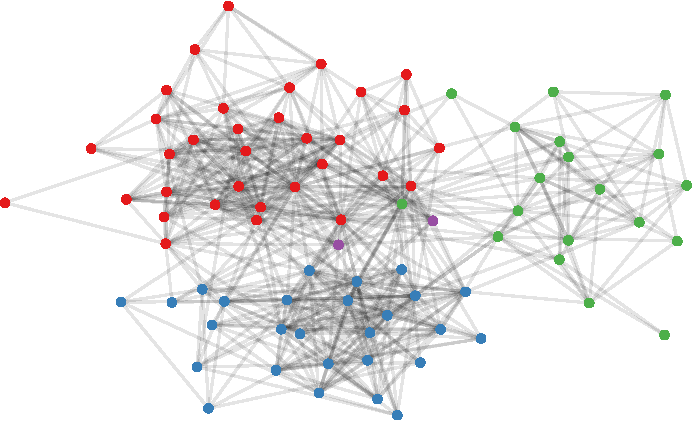
\includegraphics{draft_files/figure-latex/friendship-network-1} 

}

\caption{Friendship network of 81 faculty at a UK university. The vertices are labeled by school affiliation.}\label{fig:friendship-network}
\end{figure}
\end{example}

\hypertarget{probabilistic-models-for-graphs}{%
\subsection{Probabilistic Models for Graphs}\label{probabilistic-models-for-graphs}}

Given a sample or dataset, a typical analysis task is statistical inference, or the estimation of various parameters under the assumption that the data come from a random distribution or process.
These estimated parameters are often then used for making predictions or deriving insights about the population.
For example, when fitting a Gaussian mixture model, the data are first assumed to come from a mixture of Gaussians.
The model fitting process then involves estimating the means and standard deviations of each Gaussian component, along with the mixture weights.
The resulting model provides insight into where each mixture component is located, how disperse each component is, and how the data are distributed between the components, as well as a prediction indicating to which mixture a new observation belongs.
In order to perform a similar type of analysis for graphs, we must first define probability distributions from which such data can be sampled.

Within the scope of this work, we focus primarily on unweighted and undirected graphs without self-loops, with a brief discussion on generalizing these methods to weighted or directed graphs.
The adjacency matrix that describes these graphs is binary, symmetric, and hollow.
In this setting, a plausible model is to sample each edge independently from a Bernoulli distribution, i.e., \(A_{ij} \indep \Bernoulli(P_{ij})\) for some \(P_{ij} \in [0, 1]\) for each \(i < j\) (setting \(A_{ji} = A_{ij}\) since \(A\) is symmetric, and \(A_{ii} = 0\) since \(A\) is hollow).
Then similar to how the edges are compiled into an adjacency matrix \(A\), the edge probabilities can be compiled into an edge probability matrix \(P \in [0, 1]^{n \times n}\).
This type of graph model is defined as a \emph{Bernoulli graph} (also called an inhomogeneous \(\ER\) graph).
If \(A\) is the adjacency matrix of a Bernoulli graph with edge probability matrix \(P\), we denote \(A \sim \BG(P)\).
If the vertices and edge probabilities are sampled as a sequence of \(n\) i.i.d. random variables from probability distribution \(F\), then we denote \(A \sim \BG(F, n)\).

Statistical inference is not possible on a general Bernoulli graph with arbitrary edge probabilities since the number of parameters (individual edge probabilities) is equal to the number of observations (presence or absence of an edge).
Additional structure must be introduced.
One such structured Bernoulli graph model is the \(\ER\) graph, first proposed by \cite{Gilbert:1959}, which is defined as follows:

\begin{definition}[$\ER$ graph]
\label{def:erdos-renyi}
Let $P$ be an $n \times n$ matrix such that each $P_{ij} \equiv \theta \in [0, 1]$ is a constant. 
Then $A \sim \BG(P)$ is an $\ER$ graph. 
\end{definition}

\begin{example}[Maximum likelihood estimator for the $\ER$ graph]
One possible estimator for the lone parameter of an $\ER$ graph, $\theta$, is the maximum likelihood estimator, which is found by maximizing the log-likelihood function $\ell(\theta; A) = \log \theta \sum\limits_{i < j} A_{ij} + \log (1 - \theta) \sum\limits_{i < j} (1 - A_{ij})$. 
This can be solved directly by setting $\frac{d \ell}{d \theta} = 0$, which yields $\hat{\theta} = \frac{2 |E|}{n (n-1)}$.
\end{example}

\(\ER\) graphs lie on the opposite end of the spectrum in that they restrict the model to a single parameter, which does not result in a very interesting model or reflect many networks observed in real data.
Much work has been done in developing various Bernoulli graph models that strike a balance between structure and flexibility.
Two common types of structure for graph models, that are of particular interest in this work, are edge probabilities based on latent communities \citep{doi:10.1080/0022250X.1971.9989788, NIPS2008_3578, Karrer_2011, 307cbeb9b1be48299388437423d94bf1}, called \emph{block models}, and edge probabilities based on positions in a latent space \citep{10.1007/978-3-540-77004-6_11, rubindelanchy2017statistical}, called \emph{latent space models}.

\textbf{{[}Maybe insert something here about the exponential family of random graph models and how, like mixture distributions, block models do not fit within this family?{]}}

\begin{example}
Consider a graph in which the vertices represent a collection of $n$ planets with intelligent life sending out radio waves, and the existence of an edge between vertices $i$ and $j$ represents whether planets $i$ and $j$ have established contact.  
Since radio waves decay according to the inverse-square law, a plausible model for the edge probability between two vertices is 
$$P_{ij} = \frac{C \omega_i \omega_j}{d_{ij}^2}$$ 
where $\omega_i$ is the $i^{th}$ planet's radio signal strength, $d_{ij}$ is the Euclidean distance between planets $i$ and $j$, and $C$ is a normalizing constant. 
Let $P$ be the $n \times n$ matrix of these edge probabilities. 
Then $A \sim \BG(P)$ represents the network of planets that have made contact. 

To estimate $\omega = \begin{bmatrix} \omega_1 & \cdots & \omega_n \end{bmatrix}^\top$ after observing $A$ and supposing that the relative locations of the planets as well as the normalizing constant $C$ are known, one approach might be maximum likelihood maximization. 
For simplicity, set $C = 1$. 
Then the log-likelihood function can be written as:
$$
\ell(\omega) = 
\sum_{i < j} A_{ij} \log \bigg( \frac{\omega_i \omega_j}{d_{ij}^2 -
\omega_i \omega_j} \bigg) + \log (d_{ij}^2 - \omega_i \omega_j) + const.
$$
The partial derivatives with respect to each $\omega_i$ are:
$$
\frac{\partial \ell}{\partial \omega_i} = \sum_{j \neq i} \frac{A_{ij}}{\omega_i} - \frac{\omega_j (1 - A_{ij})}{d_{ij}^2 - \omega_i \omega_j}.
$$
Setting the gradient to zero yields $n$ equations with $n$ unknowns, but it is not entirely obvious how to solve this system of equations. 
Alternatively, we can use gradient ascent or some other numerical optimization method, since this particular log-likelihood function is concave. 
\end{example}

\hypertarget{contributions-of-this-work}{%
\subsection{Contributions of this work}\label{contributions-of-this-work}}

In this work, we explore three types of block models, the stochastic block model, the degree corrected block model, and the popularity adjusted block model, as well as a family of latent space models called generalized random dot product graphs.
The contributions of this work are as follows.
First, we show that, similar to how the stochastic block model and degree corrected block model are generalized random dot product graphs with specific latent structures, the popularity adjusted block model is also a generalized random dot product graph with a specific structure.
Using estimators with well-established consistency properties for the generalized random dot product graph, we develop consistent community detection and parameter estimation algorithms for the popularity adjusted block model.

\newpage

\hypertarget{sec:blockmodel}{%
\section{Block Models for Community Detection}\label{sec:blockmodel}}

Network analysis is often concerned with community detection.
This has motivated statisticians to develop random graph models with inherent community structure in which the probability of an edge between vertices \(i\) and \(j\) depend on the communities to which vertices \(v_i\) and \(v_j\) belong.
More formally, one assigns each vertex \(v_i\) a community label \(z_i\) and assumes a Bernoulli graph in which \(P_{ij} = g(z_i, z_j, \theta_i, \theta_j)\) for some function \(g: \{1, ..., K\}^2 \times \mathbb{R}^d \times \mathbb{R}^d \to [0, 1]\) and \(\theta_i \in \mathbb{R}^d\) is a vector of real-valued parameters associated with each vertex.
Within the context of this work, we will call such models \emph{block models}.
This type of model frmaework allows us to frame the goal of community detection as a statistical inference problem:
identify the true community labels, up to permutation of the labels.

In this section, we explore the three main types of block models:
the stochastic block model \citep{doi:10.1080/0022250X.1971.9989788}, the degree corrected block model \citep{Karrer_2011}, and the popularity adjusted block model \citep{307cbeb9b1be48299388437423d94bf1}.
The main focus is on how these models are connected, particularly in how they are nested models \citep{Noroozi2022}, as well as community detection and parameter estimation via likelihood maximization.
We will later return to these block models and the relationship to another class of random graph models in sections \ref{sec:grdpg} and \ref{sec:pabm-grdpg}.

\hypertarget{sec:sbm}{%
\subsection{The Stochastic Block Model}\label{sec:sbm}}

The stochastic block model (SBM) \citep{doi:10.1080/0022250X.1971.9989788} is the simplest of the three block models and assumes that each pair of communities has a constant edge probability \(\theta_{k \ell}\).
We now give the formal definition of the SBM within the context of Bernoulli graphs:

\begin{definition}[Stochastic block model]
\label{def:sbm}
Let $G = (V, E)$ be a Bernoulli graph with $n$ vertices, described by random adjacency matrix $A$. 
Let $K \geq 1$ be an integer and $\theta_{k \ell} \in [0, 1]$ for each $k, \ell \in \{1, ..., K\}$ (if $G$ is undirected, then $\theta_{k \ell} = \theta_{\ell k}$). 
Let $z_1, ..., z_n \in \{1, ..., K\}$ be community labels associated with each vertex. 
If the edge probability matrix $P$ for this graph is such that 
$P_{ij} = \theta_{z_i, z_j}$ and $A \sim \BG(P)$, then $G$ is a stochastic block model. 
\end{definition}

There are a few conventions for exactly how a graph is sampled as an SBM.
Within the context of this work, we assume that for a particular SBM, the number of communities, \(K\), and the community edge probabilities, \(\theta_{k \ell}\), are fixed.
Then some possible ways of sampling from an SBM are as follows:

\begin{enumerate}
\def\labelenumi{\arabic{enumi}.}
\tightlist
\item
  Assume the size of the graph \(n\) is fixed.
  Then each vertex \(v_i\) has a label \(z_i\), and the edge probability matrix \(P\) is fixed.
\item
  We sample the vertices and edges in sequence and suppose that each vertex \(v_i\) comes with a label \(z_i\), which determines its edge probabilities to the other vertices.
\item
  The vertices are sampled in sequence, and each \(z_i\) is sampled as \(z_1, ..., z_n \iid \Multinomial(\alpha_1, ..., \alpha_K)\), \(\sum_k^K \alpha_k = 1\). The edge probabilities are then determined by the sample \(\{z_i\}\) and the parameters \(\{\theta_{k \ell}\}\)
\end{enumerate}

An extension to these sampling schema include Bayesian models, e.g., each \(\theta_{k \ell}\) is sampled from a distribution with support \([0, 1]\).

\begin{example}[Stochastic block model with $K = 2$ communities]
\label{ex:assort-sbm}
We construct an SBM with two communities in which $\theta_{11} = 1/2$, $\theta_{12} = 1/8$, and $\theta_{22} = 1/4$. 
Note that in this example, the within-community edge probabilities are greater than the between-community edge probability. 
A realization of this graph with $n_1 = n_2 = 32$ is illustrated by figure \ref{fig:assort-sbm}.

\begin{figure}[H]

{\centering 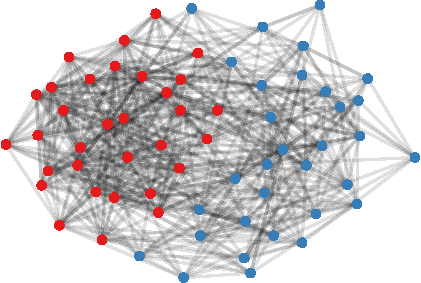
\includegraphics{draft_files/figure-latex/assort-sbm-1} 

}

\caption{Two-community stochastic block model with $\theta_{11}=1/2$, $\theta_{22}=1/4$, and $\theta_{12} = \theta_{21} = 1/8$.}\label{fig:assort-sbm}
\end{figure}
\end{example}

In most conceptions of graph models, the within-community edge probability is greater than the between-community edge probability, as in example \ref{ex:assort-sbm}.
For instance, in the UK faculty friendship network in example \ref{ex:uk-faculty}, it is natural to expect that faculty within the same school are more likely to be friends than faculty from two different schools, and a cursory look at the visualization of the graph appears to confirm this.
However, SBMs are not restricted to this type of community structure.
We could just as easily construct an example in which \(\theta_{11}\) and \(\theta_{22}\) are less than \(\theta_{12}\). Within the context of the SBM, we say that a graph is assortative if \(P\) is positive semidefinite and disassortative otherwise, which roughly correspond to communities with higher within-community edge probabilities and higher between-community edge probabilities, respectively.
For example, the SBM in example \ref{ex:assort-sbm} is assortative and has edge probability matrix \(P\) that is rank 2 with nonzero eigenvalues \(n (\frac{3}{8} \pm \frac{\sqrt{2}}{8}) > 0\).
In the following example, we describe a network which can be modeled as a disassortative SBM.

\begin{example}[Dating network as a disassortative stochastic block model]
\label{ex:sbm-dating}
Consider an undirected graph in which each vertex $v_i$ represents users of an online dating service, each label $z_i$ represents the user's gender, and each edge represents a successful match between pairs of users. 
For simplicity, we will restrict the labels to female and male (denoted as $1$ and $2$). 
If we model this as an SBM, then $\theta_{11}$ is the probability of a match between two female users, $\theta_{22}$ is the probability of a match between two male users, and $\theta_{12} = \theta_{21}$ is the probability of a match between a female user and a male user. Based on trends in the United States \citep{gallup-lgbt}, 
a plausible set of edge probabilities is $\theta_{11} = \theta_{22} = 0.02$ and $\theta_{12} = 0.2$, which are used in the sample visualized in figure \ref{fig:dating-sbm}, along with $\alpha_1 = \alpha_2 = 1/2$ and $n = 64$.

\begin{figure}[H]

{\centering 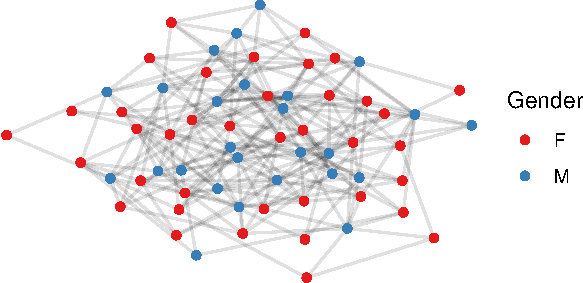
\includegraphics{draft_files/figure-latex/dating-sbm-1} 

}

\caption{Stochastic block model of a dating network. This model is disassortative.}\label{fig:dating-sbm}
\end{figure}
\end{example}

\begin{example}[Assortativity and disassortativity of the two-community SBM]
Let $P$ be the $n \times n$ probability matrix of a two-community SBM. 
Then $rank(P) = 2$, and its two nonzero eigenvalues are:

$$
\lambda = \frac{n}{2} \bigg( 
  \theta_{11} + \theta_{22} \pm 
  \sqrt{(\theta_{11} - \theta_{22})^2 + 4 \theta_{12}^2} 
\bigg).
$$
The first eigenvalue is always positive. 
The second eigenvalue is positive if $\theta_{11} \theta_{22} > \theta_{12}^2$. 
Thus, $P$ describes an assortative SBM if $\theta_{11} \theta_{22} > \theta_{12}^2$ or 
a disassortative SBM if $\theta_{11} \theta_{22} < \theta_{12}^2$. 
\end{example}

One approach to statistical inference for the SBM is likelihood maximization.
The log-likelihood function can be written as:
\begin{equation}
\label{eq:sbm-loglik}
\ell(z, \theta; A) = \sum_{i < j} \sum_{k, \ell} z_{ik} z_{j \ell} \big( 
A_{ij} \log \theta_{k \ell} - (1 - A_{ij}) \log (1 - \theta_{k \ell}) \big),
\end{equation}
where \(z_{ik} = I(z_i = k)\). If the labels are drawn from a multinomial distribution, then that can also be incorporated into the complete-data log-likelihood:
\begin{equation}
\label{eq:sbm-loglik-full}
\ell(z, \theta, \alpha; A) = \sum_k \sum_i z_{ik} \log \alpha_k + 
\sum_{i < j} \sum_{k, \ell} z_{ik} z_{j \ell} \big( 
A_{ij} \log \theta_{k \ell} - (1 - A_{ij}) \log (1 - \theta_{k \ell}) \big).
\end{equation}

The SBM is a type of mixture model, and like most classical mixture models and clustering problems, likelihood maximization is NP-hard.
Because the SBM is a mixture model, a candidate algorithm for finding a (local) maximum of the likelihood is the expectation maximization (EM) algorithm \citep{10.2307/2984875}.
However, due to the \(z_{ik} z_{j \ell}\) interaction terms, the expectation step cannot be solved in closed form \citep{kolaczyk2014statistical}.
While the labels are drawn independently, they are not necessarily conditionally independent.
Nevertheless, making the conditional independence relaxation allows us to write the expectation and maximization steps in closed form.
As an example, we write the EM algorithm for the likelihood function in equation \ref{eq:sbm-loglik} in algorithm \ref{algo:sbm-em}.

\begin{algorithm}
\label{algo:sbm-em}
  \DontPrintSemicolon
  \SetAlgoLined
  \KwData{Adjacency matrix $A$, number of communities $K$}
  \KwResult{Estimated community label probabilities $\{\pi_{ik}\}$, estimated community edge probabilities $\{\hat{\theta}_{k \ell}\}$}
  \caption{Approximate EM algorithm for the SBM}
  Initialize $\{\pi_{ik}\}$, $\{\theta_{k \ell}\}$.\;
  \While{$\|\nabla \ell\| > \epsilon$} {
    \For {$i = 1, ..., n$} {
      \For {$k = 1, ..., K$} {
        E-step: $\pi_{ik} \propto \exp \bigg( \sum_{j \neq i} \sum_{\ell} \pi_{j \ell} (A_{ij} \log \theta_{k \ell} + (1 - A_{ij}) \log (1 - \theta_{k \ell})) \bigg)$.\;
        M-step: $\theta_{k \ell} = \frac{\sum_{i < j} A_{ij} \pi_{ik} \pi_{j \ell}}{\sum_{i < j} \pi_{ik} \pi_{j \ell}}$.\;
      }
    }
  }
\end{algorithm}

Applying algorithm \ref{algo:sbm-em} to example \ref{ex:assort-sbm} with initial guesses of \(z_{ik} = 0.5\) for each \(i, k\), \(\hat{\theta}_{11} = \hat{\theta}_{22} = 0.9\), and \(\hat{\theta}_{12} = 0.1\) results in a community detection error rate of 4.7\% and parameter estimates \(\hat{\theta}_{11} = 0.503\), \(\hat{\theta}_{22} = 0.241\), and \(\hat{\theta}_{12} = 0.109\), compared to the true parameters \(\theta_{11} = 0.5\), \(\theta_{22} = 0.25\), and \(\theta_{12} = 0.125\).
The same algorithm applied to example \ref{ex:sbm-dating}, which is a disassortative model, using initial guesses of \(z_{ik} = 0.5\), \(\hat{\theta}_{11} = \hat{\theta}_{22} = 0.1\), and \(\hat{\theta}_{12} = 0.9\), results in a community detection error rate of 0\% and parameter estimates \(\hat{\theta}_{11} = 0.034\), \(\hat{\theta}_{22} = 0.018\), and \(\hat{\theta}_{12} = 0.201\), compared to the true parameters \(\theta_{11} = \theta_{22} = 0.02\) and \(\theta_{12} = 0.2\).

\hypertarget{random-graph-models-and-sparsity}{%
\subsubsection{Random Graph Models and Sparsity}\label{random-graph-models-and-sparsity}}

\hypertarget{sec:dcbm-pabm}{%
\subsection{Generalizations of the Stochastic Block Model: The Degree Corrected Block Model and the Popularity Adjusted Block Model}\label{sec:dcbm-pabm}}

\begin{definition}[Degree corrected block model]
\label{def:dcbm}
Let $G = (V, E)$ be a Bernoulli graph with $n$ vertices, described by random adjacency matrix $A$. 
Let $K \geq 1$ be an integer and $\theta_{k \ell} \in [0, 1]$ for each $k, \ell \in \{1, ..., K\}$ (if $G$ is undirected, then $\theta_{k \ell} = \theta_{\ell k}$), as in the SBM. 
Let $z_1, ..., z_n \in \{1, ..., K\}$ be community labels associated with each vertex. 
In addition, each vertex $v_i$ has a degree correction parameter $\omega_i \in [0, 1]$. 
If the edge probability matrix $P$ for this graph is such that $P_{ij} = \theta_{z_i, z_j} \omega_i \omega_j$ and $A \sim \BG(P)$, then $G$ is a degree corrected block model.
\end{definition}

\begin{example}[Dating network as a disassortative DCBM]
\label{ex:dcbm-dating}
In example \ref{ex:sbm-dating}, we modeled an online dating network as an SBM in which the vertices correspond to individuals, the communities correspond to genders, and edges correspond to whether the online dating service successfully matched pairs of individuals. 
In this model, we assume that for each pair of genders, there is a constant probability of a match. 
This does not take into account that some individuals are more likely to form connections than others. 

\end{example}

\begin{definition}[Popularity adjusted block model]
\label{def:pabm}
Let $G = (V, E)$ be an undirected Bernoulli graph with $n$ vertices, described by random adjacency matrix $A$. 
Let $K \geq 1$ be an integer that describes the number of communities, and let 
$z_1, ..., z_n \in \{1, ..., K\}$ be community labels associated with each vertex. 
Suppose that each vertex $v_i$ has $K$ popularity parameters $\lambda_{i1}, ..., \lambda_{iK}$ for which each $\lambda_{ik}$ describes $v_i$'s affinity toward community $k$. 
Then if the edge probability matrix $P$ for this graph is such that $P_{ij} = \lambda_{i, z_j} \lambda_{j, z_i}$ and $A \sim \BG(P)$, then $G$ is a popularity adjusted block model.
\end{definition}

\begin{example}[Dating network as a PABM]
\label{ex:pabm-dating}
\end{example}

\hypertarget{the-hierarchy-of-block-models}{%
\subsubsection{The Hierarchy of Block Models}\label{the-hierarchy-of-block-models}}

\newpage

\hypertarget{sec:grdpg}{%
\section{Random Dot Product Graphs and Generalized Random Dot Product Graphs}\label{sec:grdpg}}

\hypertarget{definitions}{%
\subsection{Definitions}\label{definitions}}

\begin{definition}[Generalized random dot product graph]
\label{def:grdpg}
Let $p \geq 1$ and $q \geq 0$ be integers. 
Define $I_{p,q}$ as the block diagonal matrix $I_{p,q} = \Bigl[\begin{smallmatrix} I_{p} & 0 \\ 0 & - I_{q} \end{smallmatrix} \Bigr]$ where $I_p$ and $I_q$ are the identity matrices of dimensions $p \times p$ and $q \times q$ respectively. 
Denote $d = p + q$ and let $\mathcal{X}$ be the subset of $\mathbb{R}^d$ such that, for any $x, y \in \mathcal{X}$, we have $x^\top I_{p,q} y \in [0, 1]$. 
Let $X = \begin{bmatrix} x_1 & \cdots & x_n \end{bmatrix}^\top$ be an $n \times d$ matrix with rows $x_i \in \mathcal{X}$. 
A graph $G$ with adjacency matrix $A$ is said to be a generalized random dot product graph with latent positions $X$, sparsity parameter $\rho_n$, and signature $(p, q)$ if $A \sim \BG(P)$ where the edge probability matrix $P$ is given by $P = \rho_n X I_{p,q} X^\top$, i.e., the entries of $P$ are of the form $P_{ij} = \rho_n x_i^\top I_{p,q} x_j$. 

We use the notation $A \sim \GRDPG_{p,q}(X; \rho_n)$ to denote a random adjacency matrix $A$ drawn from latent positions $X$, sparsity parameter $\rho_n$, and signature $(p, q)$. If the $n$ vectors in $X$ are drawn from probability distribution $F$ on support $\mathcal{X}$, we use the notation $A \sim \GRDPG_{p,q}(F, n; \rho_n)$. 

If $q = 0$ and so $d = p$, (i.e., $P$ is positive semidefinite), then we call this a random dot product graph. 
In this case, we use the notation $A \sim \RDPG(X; \rho_n)$ and $A \sim \RDPG(F, n; \rho_n)$. 
\end{definition}

\begin{definition}[Adjacency spectral embedding]
\label{def:ase}
\end{definition}

\begin{definition}[Indefinite orthogonal group]
\label{def:indef-ortho-group}
\end{definition}

\begin{remark}
\label{rem:non_identifiable}
The latent vectors that produce $X I_{p,q} X^\top = P$ are not unique
\citep{rubindelanchy2017statistical}.
More specifically, if $P_{ij} = x_i^\top I_{p, q} x_j$, then for any $Q \in \mathbb{O}(p, q)$ we also have 
$(Q x_i)^\top I_{p, q} (Q x_j) = x_i^\top (Q^\top I_{p, q} Q) x_j = x_i^\top I_{p, q} x_j = P_{ij}$. 
Unlike in the RDPG case, transforming the latent positions via multiplication by $Q \in \mathbb{O}(p, q)$ does not necessarily maintain interpoint angles or distances.
\end{remark}

\hypertarget{sec:sbm-dcbm-grdpg}{%
\subsection{Connecting the Stochastic Block Model and the Degree Corrected Block Model to the Generalized Random Dot Product Graph}\label{sec:sbm-dcbm-grdpg}}

\newpage

\hypertarget{sec:pabm-grdpg}{%
\section{Popularity Adjusted Block Models are Generalized Random Dot Product Graphs}\label{sec:pabm-grdpg}}

In this section, we connect the PABM to the GRDPG and exploit that connection to develop algorithms for community detection and parameter estimation.
In order to make the explicit connection between the PABM and the GRDPG, we make use of an alternative but equivalent definition of the PABM which parameterizes the model in terms of popularity vectors, which are collections of popularity parameters.

\begin{remark}
\label{rem:pabm_view2}
In a PABM, each vertex $i$ has $K$ popularity parameters $\lambda_{i1}, \dots, \lambda_{iK}$, that describe its affinity toward each of the $K$ communities. 
Another view of a PABM is as follows.
Let $\tilde{P}$ be the matrix obtained by permuting the rows and columns of $P$ so that the vertices are reorganized by community memberships $z_i \in \{1,2,\dots,K\}$ in increasing order. 
Denote by $\tilde{P}^{(k \ell)}$ the $n_k \times n_{\ell}$ submatrix of $\tilde{P}$ corresponding to the edge probabilities between vertices in communities $k$ and $\ell$. 
Here $n_k = |\{ i \colon z_i = k\}|$ is the number of vertices assigned to community $k$, for $k = 1,2\dots,K$.
Note that $\tilde{P}^{(k \ell)} = (\tilde{P}^{(\ell k)})^\top$. 
Next let $\lambda^{(k \ell)} = \{\lambda_{i \ell} \colon z_i = k\} \in \mathbb{R}^{n_k}$; the elements of $\lambda^{(k \ell)}$ are the affinity parameters toward the $\ell$th community of all vertices in the $k^{th}$ community. 
Define $\lambda^{(\ell k)}$ analogously. 
Then each block $\tilde{P}^{(k \ell)}$ can be written as the outer product of two vectors:
\begin{equation} \label{eq:pabm}
  \tilde{P}^{(k \ell)} = \rho_n \lambda^{(k \ell)} (\lambda^{(\ell k)})^{\top}.
\end{equation} 

We will henceforth use the notation \(A \sim \PABM(\{\lambda^{(k \ell)}\}_K, \rho_n)\) to denote a random adjacency matrix \(A\) drawn from a PABM with $K$ communities, popularity parameters \(\{\lambda^{(k \ell)}\}\) and sparsity parameter $\rho_n$.
\end{remark}

\hypertarget{the-geometry-of-pabms}{%
\subsection{The Geometry of PABMs}\label{the-geometry-of-pabms}}

In section \ref{sec:sbm-dcbm-grdpg}, we showed how the SBM and DCBM are special cases of the GRDPG in which the latent vectors form a very particular geometry.
Similarly, we now show the special geometry of the PABM when viewed as a GRDPG.
For ease of exposition, and without loss of generality, we drop the dependency on the sparsity parameter \(\rho_n\) and assume \(\rho_n \equiv 1\) throughout this subsection.

\begin{theorem}[The latent configuration of the PABM]
\label{thm:pabm-grdpg}
Let $A \sim \mathrm{PABM}(\{\lambda^{(k \ell)}\}_K)$ be an instance of a
PABM with $K \geq 1$ blocks and latent vectors $\{\lambda^{(k \ell)}
\colon 1 \leq k \leq K, 1 \leq \ell \leq K\}$. 
Then there exists a block diagonal matrix
$X \in \mathbb{R}^{n \times K^2}$ defined by $\{\lambda^{(k \ell)}\}$ and a 
$K^2 \times K^2$ {\em fixed} orthonormal matrix $U$ such 
that $A \sim \mathrm{GRDPG}_{K (K+1) / 2, K (K-1) /
  2}(\tilde{\Pi}XU)$. Here $\tilde{\Pi}$ is the permutation matrix
such that $P = \tilde{\Pi} \tilde{P} \tilde{\Pi}^{\top}$ where the
rows and columns of $\tilde{P}$ are arranged according to increasing values of the
community labels (see remark~\ref{rem:pabm_view2}). 
\end{theorem}

\begin{proof}
We will prove this theorem in two parts. First, for demonstration
purposes, we focus on the case when $K = 2$ to build intuition. 
The general case of $K \geq 2$ is presented later.  

For the $K = 2$ case, the proof is straightforward. We will first work with
the matrix $\tilde{P}$. Note that $\tilde{P}$ has the form

$$\tilde{P} = \begin{bmatrix} P^{(11)} & P^{(12)} \\ P^{(21)} &
  P^{(22)} \end{bmatrix} = \begin{bmatrix} \lambda^{(11)} (\lambda^{(11)})^\top & \lambda^{(12)} (\lambda^{(21)})^\top \\
  \lambda^{(21)} (\lambda^{(12)})^\top & \lambda^{(22)}
  (\lambda^{(22)})^\top \end{bmatrix}.$$
  Now let
$$X = \begin{bmatrix}
\lambda^{(11)} & \lambda^{(12)} & 0 & 0 \\
0 & 0 & \lambda^{(21)} & \lambda^{(22)}
\end{bmatrix} \quad \text{and} \quad
U = \begin{bmatrix} 1 & 0 & 0 & 0 \\
0 & 0 & 1 / \sqrt{2} & 1 / \sqrt{2} \\
0 & 0 & 1 / \sqrt{2} & - 1 / \sqrt{2} \\
0 & 1 & 0 & 0 \end{bmatrix}.$$
Then by straightforward matrix multiplication, we obtain 
$$X U I_{3, 1} U^\top X^\top =
\begin{bmatrix}
  \lambda^{(11)} (\lambda^{(11)})^\top & \lambda^{(12)} (\lambda^{(21)})^\top \\
  \lambda^{(21)} (\lambda^{(12)})^\top & \lambda^{(22)} (\lambda^{(22)})^\top
\end{bmatrix} = \tilde{P}$$
and hence $\tilde{P}$ also corresponds to the edge probability matrix of GRDPG
with latent vectors described by $X U$. As $P = \tilde{\Pi} \tilde{P}
\tilde{\Pi}^{\top}$ we conclude that $P$ has latent vectors described
by $\tilde{\Pi} X U$. 

It is nevertheless instructive to look at a few intermediate steps. 
More specifically, the product $U I_{3, 1} U^\top$ 
yields a permutation matrix $\Pi$ with fixed points at positions $1$ and $4$ 
and a cycle of order 2 swapping positions $2$ and $3$, i.e., 
$$\Pi = U I_{3, 1} U^\top = \begin{bmatrix} 1 & 0 & 0 & 0 \\
  0 & 0 & 1 & 0 \\
  0 & 1 & 0 & 0 \\
  0 & 0 & 0 & 1
\end{bmatrix}.$$
Furthermore, as $U$ is orthonormal and $I_{3, 1}$ is diagonal, 
$U I_{3, 1} U^\top$ is also an eigendecomposition of $\Pi$ where the fixed
points of $\Pi$ are mapped to the eigenvectors $e_1$ and $e_4$
while the cycles of order two are mapped to the eigenvectors  
$\tfrac{1}{\sqrt{2}}(e_{2} + e_3)$ and $\tfrac{1}{\sqrt{2}}(e_{2} -
e_3)$; here $e_i$ denote the $i^\mathrm{th}$ basis vector in $\mathbb{R}^{4}$. 
Thus, another way of decomposing the edge probability matrix is
$\tilde{P} = X \Pi X^\top$ where the rows of $X$ lie in the union of
two 2-dimensional orthogonal subspaces and $\Pi$ is a permutation matrix. 

For the general case, we can extend $\tilde{P} = X \Pi X^\top$ to larger $K$. 
For a more concrete example of this, refer to Example~1. 
We once again consider $\tilde{P}$ as defined in
remark~\ref{rem:pabm_view2}.  
We first define the following matrices

\begin{gather}
\label{eq:xy}
\Lambda^{(k)} = \begin{bmatrix} \lambda^{(k1)} \mid \cdots \mid \lambda^{(kK)} \end{bmatrix}
\in \mathbb{R}^{n_k \times K}, \quad
X = \mathrm{blockdiag}(\Lambda^{(1)}, \dots, \Lambda^{(K)}) \in
\mathbb{R}^{n \times K^2}, \\
L^{(k)} = \mathrm{blockdiag}(\lambda^{(1k)}, \dots, \lambda^{(Kk)}) \in
\mathbb{R}^{n \times K}, \quad
Y = \begin{bmatrix} L^{(1)} \mid \cdots \mid L^{(K)} \end{bmatrix} \in
\mathbb{R}^{n \times K^2}.
\end{gather}

It is then straightforward to verify that

\begin{gather*}
  XY^{\top} = \mathrm{blockdiag}(\Lambda^{(1)}, \dots,
\Lambda^{(K)}) \begin{bmatrix} L_1^{\top} \\ \vdots \\
  L_{K}^{\top} \end{bmatrix} = \begin{bmatrix} \Lambda^{(1)}
  (L^{(1)})^{\top} \\ \vdots \\
  \Lambda^{(K)} (L^{(K)})^{\top} \end{bmatrix}, \\
\Lambda^{(k)} (L^{(k)})^{\top} = \begin{bmatrix} \lambda^{(k1)}
  (\lambda^{(1k)})^{\top} \mid \dots \mid \lambda^{(kK)}
  (\lambda^{(Kk)})^{\top} \end{bmatrix} = \begin{bmatrix} P^{(k1)}
  \mid P^{(k2)} \mid \dots \mid P^{(kK)} \end{bmatrix}.
\end{gather*}
We therefore have $\tilde{P} = X Y^\top$. 
Similar to the $K = 2$ case, we also have $Y = X \Pi$ for some permutation matrix
$\Pi$ and hence $\tilde{P} = X \Pi X^\top$.
The permutation described by $\Pi$ now has $K$ fixed points, which correspond to
$K$ eigenvalues equal to $1$ with corresponding eigenvectors $e_k$ where
$k = r (K + 1) + 1$ for $0 \leq r \leq K - 1$. It also has
$\tbinom{K}{2}$ cycles of order $2$. Each cycle corresponds to
a pair of eigenvalues $\{-1,+1\}$ and a pair of eigenvectors
$\{(e_s + e_t)/\sqrt{2},(e_s - e_t)/ \sqrt{2}\}$. 

Let $p = K (K + 1) / 2$ and $q = K (K - 1) / 2$. 
We therefore have
\begin{equation} \label{eq:permutation}
\Pi = U I_{p,q} U^\top
\end{equation}
where $U$ is a $K^2 \times K^2$ orthogonal matrix and hence
\begin{equation} \label{eq:pabm-grdpg}
\tilde{P} = X U I_{p, q} (X U)^\top.
\end{equation}
In summary we can describe the PABM with $K$ communities as a GRDPG with latent
positions $\tilde{\Pi} X U$ and known signature $(p,q) = \bigl( \tfrac{1}{2} K (K + 1) ,
\tfrac{1}{2} K (K - 1)\bigr)$.
\end{proof}

\begin{example} Let $A$ be a $3$ blocks PABM with latent vectors $\{\lambda^{(k \ell)} \colon 1 \leq k \leq 3, 1 \leq \ell \leq 3\}$. 
Using the same notation as in theorem~\ref{thm:pabm-grdpg}, we can define
\begin{gather*}
X = \begin{bmatrix}
\lambda^{(11)} & \lambda^{(12)} & \lambda^{(13)} & 0 & 0 & 0 & 0 & 0 & 0 \\
0 & 0 & 0 & \lambda^{(21)} & \lambda^{(22)} & \lambda^{(23)} & 0 & 0 & 0 \\
0 & 0 & 0 & 0 & 0 & 0 & \lambda^{(31)} & \lambda^{(32)} & \lambda^{(33)}
\end{bmatrix}, \\
Y = \begin{bmatrix}
\lambda^{(11)} & 0 & 0 & \lambda^{(12)} & 0 & 0 & \lambda^{(13)} & 0 & 0 \\
0 & \lambda^{(21)} & 0 & 0 & \lambda^{(22)} & 0 & 0 & \lambda^{(23)} & 0 \\
0 & 0 & \lambda^{(31)} & 0 & 0 & \lambda^{(32)} & 0 & 0 & \lambda^{(33)}
\end{bmatrix}.
\end{gather*}
Then $Y = X \Pi$ and $\tilde{P} = X Y^{\top}$ where $\Pi$ is a $9 \times 9$ 
permutation matrix of the form
$$\Pi = 
\Bigl[e_1 \mid e_4 \mid e_7 \mid e_2 \mid e_5 \mid e_8 \mid e_3
\mid e_6 \mid e_9 \Bigr].$$
where $e_i$ denotes the $i^{th}$ basis vector in $\mathbb{R}^{9}$. 
The matrix $\Pi$ corresponds to a permutation of $\{1,2,\dots,9\}$ with the following decomposition.
\begin{enumerate}
\item Positions 1, 5, 9 are fixed.
\item There are three cycles of length 2, namely $(2, 4)$, $(3, 7)$, and $(6, 8)$.
\end{enumerate}
We can thus write $\Pi$ as $\Pi = U I_{6, 3} U^\top$ where the first three columns of $U$ consist of $e_1$, $e_5$, and $e_9$ corresponding to the fixed points, the next three columns are the eigenvectors $(e_k + e_{\ell}) / \sqrt{2}$, and the last three columns are the eigenvectors $(e_k - e_{\ell}) / \sqrt{2}$ for $(k, \ell) \in \{(2,4),(3,7),(6,8)\}$.

The matrix $\tilde{P}$ is then the edge probabilities matrix for a 
Generalized Random Dot Product Graph whose latent positions 
are the rows of the matrix
$$XU = \begin{bmatrix}
  \lambda^{(11)} & 0 & 0 &
  \frac{\lambda^{(12)}}{\sqrt{2}} & \frac{\lambda^{(13)}}{\sqrt{2}} & 0 &
  \frac{\lambda^{(12)}}{\sqrt{2}} & \frac{\lambda^{(13)}}{\sqrt{2}} & 0 \\
  0 & \lambda^{(22)} & 0 &
  \frac{\lambda^{(21)}}{\sqrt{2}} & 0 & \frac{\lambda^{(23)}}{\sqrt{2}} &
  -\frac{\lambda^{(21)}}{\sqrt{2}} & 0 & \frac{\lambda^{(23)}}{\sqrt{2}} \\
  0 & 0 & \lambda^{(33)} &
  0 & \frac{\lambda^{(31)}}{\sqrt{2}} & \frac{\lambda^{(32)}}{\sqrt{2}} &
  0 & -\frac{\lambda^{(31)}}{\sqrt{2}} & -\frac{\lambda^{(32)}}{\sqrt{2}}
\end{bmatrix}$$
and the latent positions for $P$ is a permutation of the rows of
$XU$. 
\end{example}

\hypertarget{algorithms}{%
\subsection{Algorithms}\label{algorithms}}

Two inference objectives arise from the PABM:

\begin{enumerate}
\def\labelenumi{\arabic{enumi}.}
\tightlist
\item
  Community membership identification (up to permutation).
\item
  Parameter estimation (estimating $\lambda_{ik}$'s).
\end{enumerate}

In our methods, the data that are observed for estimation is the adjacency matrix, \(A \sim \PABM(\{\lambda^{(k \ell)}\}_K, \rho_n)\), along with an assumed number of communities, \(K\).
To motivate our methods, we first consider community detection and parameter estimation in the case where we know the edge probability matrix \(P\) beforehand, noting that community memberships and popularity parameters are not immediately discernible from \(P\) itself.
After establishing methods for community detection and parameter estimation from \(P\), we use the consistency property of the ASE \citep{doi:10.1080/01621459.2012.699795,rubindelanchy2017statistical} to demonstrate that the same methods work for \(A\) almost surely as \(n \to \infty\).

\hypertarget{previous-work}{%
\subsubsection{Previous Work}\label{previous-work}}

\citet{307cbeb9b1be48299388437423d94bf1}
used Modularity Maximization (MM) and the Extreme Points (EP)
algorithm \citep{le2016} for community detection and parameter
estimation. They were able to show that as the sample size increases,
the \emph{proportion} of misclassified community labels (up to permutation)
goes to 0.

\cite{noroozi2019estimation} used Sparse Subspace Clustering (SSC)
\citep{5206547} for community detection in the PABM.
The SSC algorithm can be described as follows:
Given \(X \in \mathbb{R}^{n \times d}\) with vectors
\(x_i^\top \in \mathbb{R}^d\) as rows of \(X\), the optimization problem
\(c_i = \argmin_{c} \|c\|_1\) subject to \(x_i = X^\top c\) and
\(c^{(i)} = 0\), where \(c^{(i)}\) is the \(i^{th}\) entry of \(c\), is solved for each \(i \in [n]\).
The solutions are collected into matrix
\(C = \bigl[ c_1 \mid \cdots \mid c_n \bigr]^\top\) to
construct an affinity matrix \(B = |C| + |C^\top|\). If each \(x_i\) lies
exactly on one of \(K\) subspaces, \(B\) describes an undirected graph
consisting of \emph{at least} \(K\) disjoint subgraphs, i.e., \(B_{ij} = 0\) if \(x_i, x_j\) lie on different subspaces.
The intuition here is that vectors that lie on the same subspace can be described as linear combinations of each other, assuming the number of vectors in the subspace is greater than the dimensionality of the subspace.
Then once sparsity is enforced, for each \(c_i\), its \(j^{th}\) element \(c_i^{(j)}\) is zero if \(x_j\) belongs to a subspace that doesn't contain \(x_i\), resulting in \(B_{ij} = 0\).
If \(X\) instead represents points near \(K\) subspaces with some noise,
then this property may only hold approximately and a final graph partitioning step may be required
(e.g., edge thresholding or spectral clustering).

In practice, due to presence of noise, SSC is often done by solving the LASSO problems
\begin{equation} 
\label{eq:ssc}
c_i = \argmin_c \frac{1}{2} \|x_i - X_{-i}^\top c\|^2_2 + \vartheta \|c\|_1
\end{equation}
for some sparsity parameter \(\vartheta > 0\).
The \(c_i\) vectors are then collected into \(C\) and \(B\) as before.

\begin{definition}[Subspace Detection Property]
\label{def:subspace_detection}
Let $X = \bigl[ x_1 \mid \cdots \mid x_n \bigr]^\top$ be noisy points sampled from $K$ subspaces, i.e., $x_i = y_i + z_i$ where the $y_i$ belongs to the union of $K$ subspaces and the $z_i$ are noise vectors. 
Let $\vartheta \geq 0$ be given and let $C$ and $B$ be constructed from the solutions of LASSO problems as described in equation~\ref{eq:ssc} with this given choice of $\vartheta$. 
Then $X$ is said to satisfy the subspace detection property with sparsity parameter $\vartheta$ if each column of $C$ has nonzero $\ell_2$ norm and $B_{ij} = 0$ whenever $y_i$ and $y_j$ are from different subspaces.
\end{definition}

\begin{remark}
\label{rem:sdp}
One common approach to show that SSC works for a noisy sample $X$ is to show that $X$ satisfies the subspace detection property for some choice of $\vartheta$; 
recall that $\vartheta$ is the sparsity parameter for
the LASSO problems in equation~\ref{eq:ssc}. However, this is not sufficient to
guarantee that SSC perfectly recovers the underlying subspaces.
More specifically, if $X$ satisfies the 
subspace detection property, 
then $B$ describes a graph with {\em at least} $K$ disconnected subgraphs, 
with the ideal case being that there are exactly $K$ subgraphs 
which map onto each subspace. 
Nevertheless it is also possible that the $K$ subspaces are represented by
$K' > K$
multiple disconnected subgraphs and we cannot, at least without a subsequent
post-processing step, recover the $K$ subspaces directly from $B$;
see \citet{sdp_sufficiency} and \citet{liu_ssc}
for further discussions. Therefore in practice $B$ is usually treated as an
affinity matrix and, as we allude to earlier, 
the rows of $B$ are partitioned using some
clustering algorithm to obtain the final clustering. 
\end{remark}

Theorem \ref{thm:pabm-grdpg} suggests that SSC is appropriate for community
detection for the PABM, provided that we observe the edge probabilities
matrix \(P\). More precisely, given the matrix \(\tilde{P}\) obtained by
permuting the rows and columns of \(P\) as described in
remark \ref{rem:pabm_view2} we can recover \(XU\) up
to some non-identifiability indefinite orthogonal transformation \(Q\).
Then using results from \citet{soltanolkotabi2012}, it can be easily shown
that the subspace detection property holds for \(XU\). Indeed, the columns
of \(XU\) from different communities correspond to mutually
orthogonal subspaces. This then implies that the
subspace detection property also holds for \(XUQ\) for all invertible
transformation \(Q\) and hence the subspace detection property also holds for
\(\tilde{\Pi} X U Q\) for any \(n \times n\) permutation matrix \(\tilde{\Pi}\).

However, because we do not observe \(P\) but rather only the noisy
adjacency matrix \(A \sim \BG(P)\), the natural approach then is
to perform SSC on the rows of the spectral embedding of \(A\),
since the embedding of \(P\) consists of \(K\) subspaces (theore \ref{thm:pabm-grdpg}),
and so the embedding of \(A\) will lie approximately on the \(K\) subspaces.
We will show in theorem \ref{theorem5} that, with probability converging to
one as \(n \rightarrow \infty\), the rows of the ASE of \(A\) also
satisfy the subspace detection property.
Theorem \ref{theorem5} builds upon existing work by
\citet{rubindelanchy2017statistical} who describe the convergence
behavior of the ASE of \(A\) to that of \(\tilde{\Pi} XU\), and
\citet{jmlr-v28-wang13} who show the necessary conditions for the
subspace detection property to hold in noisy cases where the points lie
near subspaces. Finally we emphasize that while
\citet{noroozi2019estimation} also considered the use of SSC for
community recovery in PABM, they instead applied SSC to the rows of
\(A\) itself, foregoing
the embedding step altogether. It is however much harder to show that
the rows of \(A\) satisfy the subspace detection property and thus, to
the best of our knowledge, there is currently no consistency result
regarding the application of SSC to the rows of \(A\).

We previously stated in theorem \ref{thm:pabm-grdpg} one possible set of latent positions that result in
the edge probability matrix of a PABM, namely
\(P = \tilde{\Pi} (XU) I_{p, q} (XU)^\top \tilde{\Pi}^{\top}\) where \(X\) is block diagonal and
\(\tilde{\Pi}\) is a permutation matrix.\\
Furthermore, the explicit form of \(XU\) represents points in \(\mathbb{R}^{K^2}\)
such that points within each community lie on \(K\)-dimensional
orthogonal subspaces, i.e.~\(\langle U^{\top} x_i, U^{\top} x_j \rangle = 0\) whenever \(i\) and \(j\) are in different communities.
Thus if we have (or can estimate) \(XU\) directly, then both the community
detection and parameter identification problem are trivial because \(U\)
is orthonormal and fixed for each value of \(K\).
However, direct
identification or estimation of \(XU\) is possibly difficult
due to the non-identifiability of \(XU\) (see remark \ref{rem:non_identifiable})
when we are given only \(P\).
More specifically, suppose we find a matrix \(Y \in \mathbb{R}^{n \times K^2}\)
such that \(P = Y I_{p, q} Y^\top\). Then it is generally the case that
\(Y = \tilde{\Pi} XU Q\) for some indefinite orthogonal matrix
\(Q \in \mathbb{O}(p,q)\).
However since \(Q\) is not necessarily an
orthogonal matrix and hence, if \(y_i\) denote the \(i^{th}\) row of \(Y\),
then \(\langle U^{\top} x_i, U^{\top} x_j \rangle \neq \langle y_i, y_j \rangle\).
This prevents us from transferring the orthogonality property of
\(XU\) directly to \(Y\).

Nevertheless by using the special geometric structure of \(X\) we can circumvent the
non-identifiability of \(Y\) and \(XU\) by using instead the rows of the
matrix \(V\) of eigenvectors (corresponding to the non-zero eigenvalues) of \(P\). In particular \(V\) is identifiable
up to orthogonal transformations and furthermore, due to the block
diagonal structure of \(X\), the rows of \(V\) also lie on \(K\) distinct orthogonal
subspaces and hence \(v_i^{\top} v_j = 0\) whenever \(z_i \not = z_j\).

\begin{theorem}
\label{thm:osc-p}
Let $P = V D V^\top$ be the spectral decomposition 
of the edge probability matrix. 
Let $B = n V V^\top$. 
Assume $\lambda_{i z_i} > 0$ for each $i \in [n]$, 
i.e., each vertex's popularity parameter to its own community is nonzero. 
Then $B_{ij} = 0$ if and only if 
vertices $i$ and $j$ are in different communities.
\end{theorem}

\begin{proof}
We first show that $V V^\top =
\tilde{\Pi} X (X^\top X)^{-1} X^\top \tilde{\Pi}^{\top} $ where $X$ is 
defined as in Eq.~\eqref{eq:xy}. Indeed, by Theorem 2, 
\(P = \tilde{\Pi} X U I_{p, q} U^\top X^\top \tilde{\Pi}\) for $p = K(K+1)/2$ and $q = K(K-1)/2$. 
The eigendecomposition \(P = V D V^\top\) also yields $P = V
|D|^{1/2} I_{p, q} |D|^{1/2} V^\top$ where \(|\cdot|^{1/2}\) is
applied entry-wise. Now let $Y = \tilde{\Pi} XU$ and $\tilde{Y} = V|D|^{1/2}$; note that
$Y$ and $\tilde{Y}$ both have full column ranks. 
Because $P = Y I_{p,q} Y^{\top} = \tilde{Y} I_{p,q} \tilde{Y}^{\top}$, we have
$$Y = \tilde{Y} I_{p,q} \tilde{Y}^{\top} Y (Y^{\top} Y)^{-1} I_{p,q}.$$
Let $Q = I_{p,q} \tilde{Y}^{\top} Y (Y^{\top} Y)^{-1} I_{p,q}$ and note that
$Y = \tilde{Y} Q$. We then have
\begin{equation*}
  \begin{split}
  Q^{\top} I_{p,q} Q &= I_{p,q} (Y^{\top} Y)^{-1} Y^{\top} \tilde{Y} I_{p,q}
I_{p,q} I_{p,q} \tilde{Y}^{\top} Y (Y^{\top} Y)^{-1} I_{p,q} \\ 
&= I_{p,q} (Y^{\top} Y)^{-1} Y^{\top} Y I_{p,q}
Y^{\top} Y (Y^{\top} Y)^{-1} I_{p,q} =  I_{p,q}
\end{split}
\end{equation*}
and hence $Q$ is an indefinite orthogonal matrix. 

Let $R = U Q |D|^{-1/2}$ and note that $V = \tilde{\Pi} XR$. Because $R$ is
invertible, we can write
$$\tilde{\Pi} X (X^{\top} X)^{-1} X^{\top} \tilde{\Pi}^{\top} =
\tilde{\Pi} X R (R^{\top} X^{\top} X R)^{-1}
R^{\top} X^{\top} \tilde{\Pi}^{\top}.$$ 
Furthermore, as $V$ has orthonormal columns, $R^{\top} X^{\top} X R =
V^{\top} \tilde{\Pi} \tilde{\Pi}^{\top} V = V^{\top} V = I$. We thus conclude
$$\tilde{\Pi} X (X^{\top} X)^{-1} X^{\top} \tilde{\Pi}^{\top} = V (V^{\top} V)^{-1} V^{\top} = V V^{\top}$$
as desired.

To complete the proof of theorem \ref{thm:osc-p}, recall that \(X\) 
is block diagonal with each block corresponding to one community, 
and hence \(X (X^\top X)^{-1} X^\top\) is also a
block diagonal matrix with each block corresponding to a community. 
As $B = n VV^{\top} = n \tilde{\Pi} X (X^\top X)^{-1} X^\top \tilde{\Pi}^{\top}$, 
we conclude that $B_{ij} = 0$ 
whenever vertices $i$ and $j$ belong to different communities.  
\end{proof}

Theorem \ref{thm:osc-p} provides perfect community detection from \(P\).
More specifically, let \(|B|\) be the affinity matrix for graph \(G'\),
where \(|\cdot|\) is applied entry-wise. Then
\(G'\) consists of exactly \(K\) disjoint subgraphs,
as \(G'\) has no edges between communities.
All that is left to identify the communities is
to assign each subgraph a distinct community label.
In practice, we do not observe \(P\) and instead only observe the noisy
\(A \sim \BG(P)\). A natural approach is then to use
the affinity matrix \(\hat{B} = n \hat{V} \hat{V}^{\top}\) where
\(\hat{V}\) is the matrix of eigenvectors (corresponding to the largest
eigenvalues in modulus) of \(A\). The resulting procedure, named
Orthogonal Spectral Clustering, is presented in
algorithm \ref{alg:osc}.
The following result leverages existing theoretical properties
of ASE for estimating of latent positions in a GRDPG \citep{rubindelanchy2017statistical} to show that
\(\hat{B}\) converges almost surely to \(B\); in particular
\(\hat{B}_{ij} \stackrel{a.s.}{\to} 0\)
for each pair \((i, j)\) in different communities.

\begin{algorithm}[tp]
  \label{alg:osc}
  \DontPrintSemicolon
  \SetAlgoLined
  \KwData{Adjacency matrix $A$, number of communities $K$}
  \KwResult{Community assignments $1, ..., K$}
    Compute the eigenvectors of $A$ that correspond to the $K (K+1) / 2$ most
    positive eigenvalues and $K (K-1) / 2$ most negative eigenvalues. Construct
    $V$ using these eigenvectors as its columns.\;
    Compute $B = |n V V^\top|$, applying $|\cdot|$ entry-wise.\;
    Construct graph $G$ using $B$ as its similarity matrix.\;
    Partition $G$ into $K$ disconnected subgraphs
    (e.g., using edge thresholding or spectral clustering).\;
    Map each partition to the community labels $1, ..., K$.\;
  \caption{Orthogonal Spectral Clustering.}
\end{algorithm}

\begin{theorem}
\label{thm:osc}
Assume the setting of theorem \ref{thm:osc-p}. 
Let $\hat{B}$ with entries $\hat{B}_{ij}$ be the affinity matrix
obtained from OSC as described in algorithm~\ref{alg:osc}. 
Then for $n \rho_n = \omega(\log^{4}{n})$, we have
\begin{equation} 
\label{eq:osc}
\max_{i, j} |\hat{B}_{ij} - B_{ij}| = O\Big( \frac{\log n}{\sqrt{n \rho_n}} \Big)
\end{equation}
with high probability. In particular 
$\hat{B}_{ij} -B_{ij} \overset{\mathrm{a.s.}}{\rightarrow} 0$ 
where the convergence is
uniform over all $i,j$. Hence for all pairs $(i,j)$ in different
communities we have 
$\hat{B}_{ij} \overset{\mathrm{a.s.}}{\rightarrow} 0$, 
while for all pairs $(i, j)$ in the same community, 
$\liminf_{n \to \infty} |\hat{B}_{ij}| > 0$ almost surely. 
\end{theorem}

\newpage

\hypertarget{generalized-random-dot-product-graphs-with-community-structure}{%
\section{Generalized Random Dot Product Graphs with Community Structure}\label{generalized-random-dot-product-graphs-with-community-structure}}

\newpage

\section*{Appendix A: Proofs of Theorems}

Let \(V_n\) and \(\hat{V}_n\)
be the \(n \times K^2\) matrices whose columns are the eigenvectors of \(P\) and \(A\) corresponding to the
\(K^2\) largest eigenvalues (in modulus), respectively.
We first state an important technical lemma for bounding the maximum
\(\ell_2\) norm difference between the rows of \(\hat{V}_n\) and
\(V_n\). See \citet{cape_biometrika} and
\citet[Lemma~5]{rubindelanchy2017statistical} for a proof.

\begin{lemma}
\label{lem:technical}
Let $A \sim \mathrm{PABM}(\{\lambda^{(k \ell \ell)}\}_{K})$ be a $K$-blocks
PABM graph on $n$ vertices and let \(V\) and \(\hat{V}\)
be the $n \times K^2$ matrices whose columns are the eigenvectors of 
\(P\) and \(A\) corresponding to the
$K^2$ largest eigenvalues in modulus, respectively.
Let \(v_i^\top\) and \(\hat{v}_i^\top\) denote the $i$th 
row of \(V\) and \(\hat{V}\), respectively. 
Then there exists a constant $c > 1$ and an orthogonal matrix $W$ such
that with high probability,
$$\max_{i} \|W \hat{v}_i - v_i\|  = O\Big(\frac{\log^{c}n}{n \sqrt{\rho_n}} \Big).$$
In particular we can take $c = 1 + \epsilon$ for any $\epsilon > 0$. 
\end{lemma}

\begin{proof}[Proof of theorem~\ref{thm:osc}]
Recall the notations in lemma~\ref{lem:technical} and note that,
under our assumption that the latent vectors $\lambda^{(k \ell)}$
are all homogeneous, we have $\max_{i} \|v_i\| =
O(n^{-1/2})$. 

Next recall theorem~\ref{thm:osc-p}; in particular $B_{ij} = nv_i^{\top}
v_j$. 
We therefore have
\[\begin{split}
 \max_{ij} |\hat{B}_{ij} - B_{ij}| &= \max_{ij} n |\hat{v}_i^\top \hat{v}_j -
v_i^\top v_j| \\
& \leq n \max_{ij} |\hat{v}_i^\top W W^\top \hat{v}_j -
v_i^\top v_j| \\
& \leq n \max_{i,j} \Bigl(\|W^{\top} \hat{v}_i - v_i\| \times \|\hat{v}_j\|
+ \|W^{\top} \hat{v}_j - v_j\| \times \|v_i\|\Bigr) \\
& \leq n \Bigl(\max_{ij}  \|W \hat{v}_i  - v_i \|^2 +  \|W
\hat{v}_i  - v_i \| \times \|v_j\| +  \|W \hat{v}_j  - v_j \| \times \|v_i\|\Bigr) 
\\ &
\leq n \max_{i} \|W \hat{v}_i  - v_i \|^2 + 2n \max_{i}
\|W \hat{v}_i  - v_i \| \times \max_{j} \|v_j\|
\\
& = O \Big( \frac{\log^{c}{n}}{n^{1/2} \rho_n^{1/2}} \Big)
\end{split}\]
with high probability.
Theorem~\ref{thm:osc} follows from the above bound together with the
conclusion in theorem~\ref{thm:osc-p} that $B_{ij} = 0$ whenever vertices $i$ and $j$
belongs to different communities. 
\end{proof}

\newpage

\renewcommand\refname{References}
  \bibliography{bibliography.bib}

\end{document}
